\chapter{Математическая модель движения мобильных плавающих роботов}\label{ch:ch2}

\section{Описание математчиеской модели движения мобильного робота в форме эллипсоида в жидкости}\label{sec:ch2/sec1}

Рассмотрим систему, состоящую из жесткой внешней оболочки и трех внутренних роторов (рисунок \ref{rotors}). Геометрический центр системы совпадает с центром сферической части оболочки.

\begin{figure}[th]
	\begin{center}
		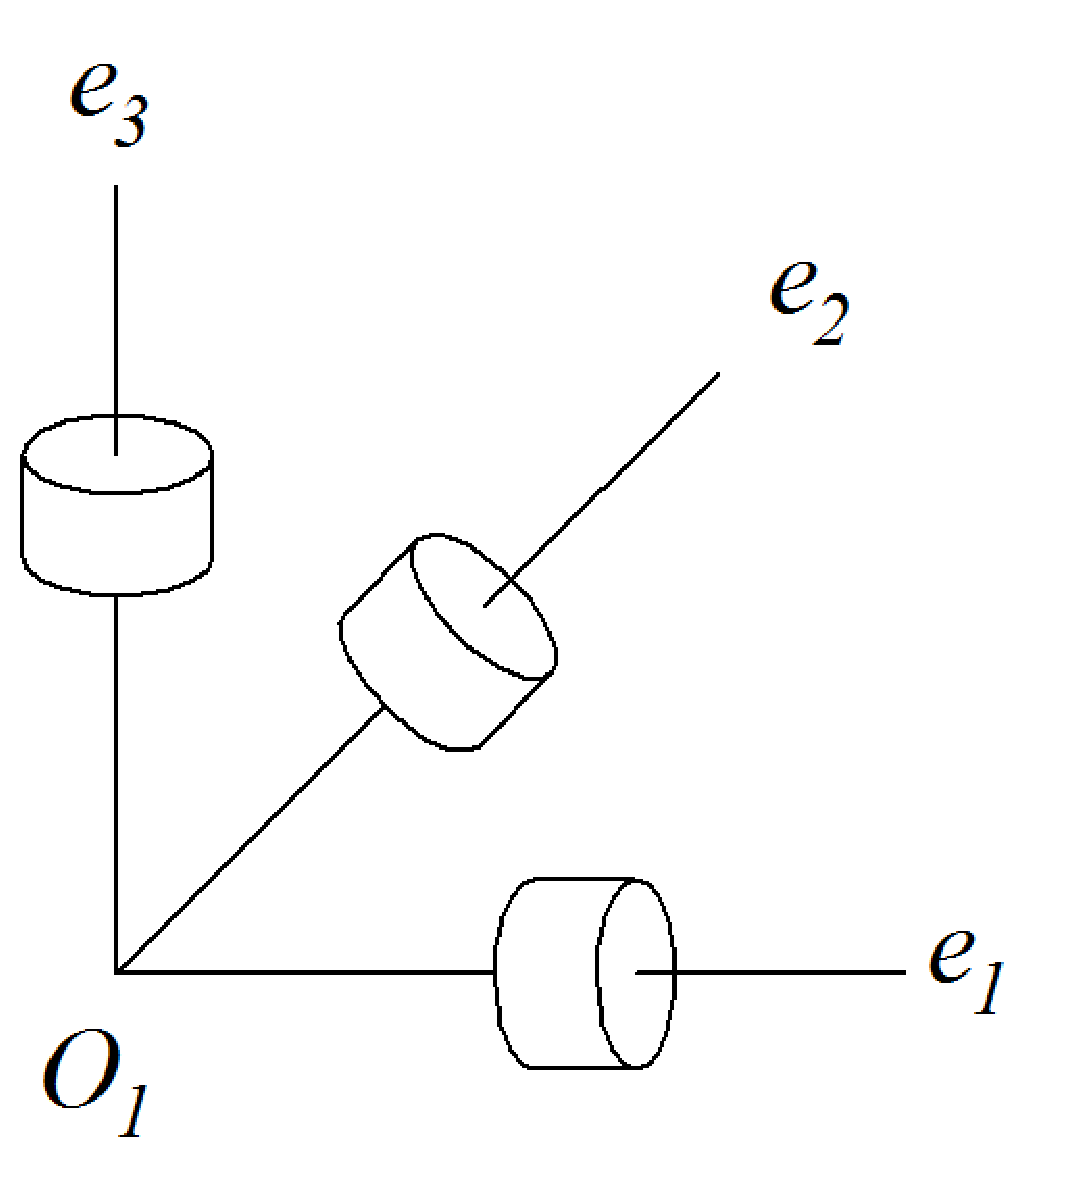
\includegraphics[width=0.3\linewidth]{rotors1.eps}
		\caption{Расположение роторов} \label{rotors}
	\end{center}
\end{figure}


Будем полагать, что конструкция удовлетворяет ряду условий:
\begin{enumerate}
	\item Оболочка является однородной, положение ее центра масс совпадает с геометрическим центром оболочки.
	%\item Центр масс всей системы находится не в геометрическом центре оболочки;
	\item Все роторы одинаковы, осесимметричны и оси вращения  совпадают с их осями симметрии, то есть вращение не изменяет распределение масс системы;
	%\item Ось вращения одного из роторов совпадает с осью винтовой симметрии оболочки;
	\item Оси вращения роторов взаимно перпендикулярны, а их угловые скорости являюся заданными функциями времени $\omega _k \bigl( t \bigr),~k=1,2,3$.
\end{enumerate}

Выберем подвижную систему координат $O_1 e_1 e_2 e_3$, жестко связанную с оболочкой, так что оси совпадают с главными осями инерции оболочки. Обозначим через $\bV$ и ${\bOm}$ скорость центра оболочки и его угловую скорость (все векторы, если не оговорено обратное, проецируются на подвижные оси).

Определим дополнительно неподвижную систему координат $O x y z$ и обозначим $\br = \bigl( x,\, y,\, z \bigr)$ -- координаты геометрического центра оболочки в этих осях. Обозначим также через ${\bal}$, ${\bbe}$, ${\bga}$ орты неподвижных осей $O x y z$, спроецированные на подвижные оси $e_1$, $e_2$, $e_3$, тогда ортогональная матрица
\begin{gather}
\bbQ =\begin{pmatrix}
\alpha _1 & \beta _1 & \gamma _1\\
\alpha _2 & \beta _2 & \gamma _2\\
\alpha _3 & \beta _3 & \gamma _3
\end{pmatrix}\nonumber \in SO(3)
\end{gather}

характеризует ориентацию тела, а пара $\left( \br,\, \bm{Q} \right)$ однозначно определяет конфигурацию системы. Таким образом, конфигурационное пространство системы шестимерно и представляет собой $\mathbb{R}^3 \times SO(3)$.

Обозначим через $m_s$ -- массу оболочки, ${\bm I}_s$ -- ее центральный тензор инерции,
\begin{gather}
\bLam = \begin{pmatrix}
\bLam _1 & 0 \\
0 & \bLam _2
\end{pmatrix}\nonumber
\end{gather}
-- матрицу коэффициентов присоединенных масс в системе $O e_1 e_2 e_3$, где $\bLam_1$ -- тензор присоединенных масс, $\bLam_2$ -- тензор присоединных моментов инерции. Тогда выражение для кинетической энергии оболочки примет вид
\begin{gather}
T_s = \frac{1}{2} m_s  \bigl( \bV,\, \bV \bigr) + \frac{1}{2} \bigl( {\bm I}_s {\bOm},\, {\bOm} \bigr),\nonumber
\end{gather}
а выражение кинетической энергии жидкости
\begin{gather}
T_f = \frac{1}{2} \bigl( \bLam_1 \bV,\, \bV \bigr) + \frac{1}{2} \bigl( {\bLam} _2 {\bOm},\, {\bOm} \bigr).\nonumber
\end{gather}

Обозначим через $m_R$ -- массу ротора, ${\bbI}_k$ -- центральный тензор инерции $k$-го ротора, записанный в системе координат $O' e_1 e_2 e_3$, $\bn_k$ -- орт оси вращения $k$-го ротора неподвижный в системе $O' e_1 e_2 e_3$, $\br_k$ -- радиус-вектор центра масс $k$-го ротора неподвижный в системе $O' e_1 e_2 e_3$. Тогда кинетическая энергия $k$-го ротора примет вид
\begin{gather}
T_k = \frac{1}{2} m_R \bigl( \bV + {\bOm} \times \br_k, \bV + {\bOm} \times \br_k \bigr) + \frac{1}{2}\Bigl({\bm I}_k \bigl( {\bOm} + \omega_k \bn_k \bigr), {\bOm} + \omega_k \bn_k \Bigr),\nonumber
\end{gather}

Суммарная кинетическая энергия всей системы с учетом того, что оси роторов задаются собственными векторами их тензоров инерции, то есть ${\bbI}_k \bn_k = i \bn_k$, примет вид
\begin{gather}
\label{kinetic_energy}
\begin{split}
T = & T_f + T_s + \sum _{k=1}^3 T_k = \\
= & \frac{1}{2} \bigl( {\bbI} {\bOm},\, {\bOm} \bigr) + \bigl( {\bbB} {\bOm},\, \bV \bigr) + \frac{1}{2} \bigl( {\bbC} \bV,\, \bV \bigr) + \bigl( {\bOm},\, \bK(t) \bigr) + \frac{1}{2} \sum_{k=1}^3 i \omega_k^2 (t),
\end{split}
\end{gather}
где $\bbI$ --- тензор инерции всей системы вычисленный относительно геометрического центра оболочки, матрицы $\bbB$ и $\bbC$ зависят от распределения масс и формы оболочки, $\bK(t)=\sum \limits_{k=0}^3 i \omega_k (t)\bn_k$ --- вектор гиростатического момента. Матрицы $\bbI$, $\bbB$, $\bbC$ имеют вид
\begin{gather}
{\bbI} = {\bLam}_2 + {\bbI}_s + \sum _{k=1}^3 {\bbI}_k + \frac{1}{2} m_R \sum _{k=1}^3 \bigl( \br_k^2{\bbE} - \br_k \otimes \br_k \bigr),\nonumber \\
{\bbC} = m {\bbE} + {\bLam}_1,\nonumber \\
{\bbB} = m \begin{pmatrix}\nonumber
0 & z_c & -y_c\\
-z_c & 0 & x_c\\
y_c & -x_c & 0
\end{pmatrix}\nonumber \\
m = m_s + 3 m_R,\nonumber
\end{gather}
где $x_c$, $y_c$, $z_c$ --- компоненты радиус-вектора $\br_c$ центра масс системы.

\begin{small}
	{\textbf{ Замечание.} Общее число параметров матриц $\bbC$, $\bbB$, $\bbI$ равно 21. С помощью подходящего выбора точки $O_1$ и ориентации осей $O_1 e_1 e_2 e_3$ матрицу $\bbI$ можно привести к диагональному виду, $\bbB$ -- к симметрическому, а общее число параметров будет равно 15 \cite{Borisov_Mamaev}. Исследования, которые будут проводиться в дальнейшем, будут осуществляться численно, поэтому вопрос о количестве параметров не является принципиальным.}
\end{small}

Уравнения движения рассматриваемой системы имеют вид классических уравнений Кирхгофа \cite{Borisov_Mamaev}
\begin{gather}
\label{Kirchhoff}
\frac{d}{dt} \biggl( \frac{\partial T}{\partial \bV} \biggr) + {\bOm} \times \frac{\partial T}{\partial \bV}=0, \quad \frac{d}{dt}\biggl( \frac{\partial T}{\partial {\bOm}} \biggr) + {\bOm} \times \frac{\partial T}{\partial {\bOm}} + \bV \times \frac{\partial T}{\partial \bV} = 0 \nonumber
\end{gather}
и с учетом (\ref{kinetic_energy}) могут быть записаны в виде
\begin{gather}
\label{motion_eq}
\begin{split}
{\bbC} \dot{\bV} + {\bbB} \dot{{\bOm}} = & \bigl( {\bbC} \bV + {\bbB} {\bOm} \bigr) \times {\bOm},\\
{\bbB}^T \dot{\bV} + {\bbI} \dot{{\bOm}} + \dot{\bK}(t) = & \bigl( {\bbB}^T \bV + {\bbI} {\bOm} + \bK(t) \bigr) \times {\bOm} + \bigl( {\bbC} \bV + {\bbB} {\bOm} \bigr) \times \bV = 0
\end{split}
\end{gather}

Данные уравнения необходимо дополнить уравнениями эволюции переменных $\bigl( \br,\, {\bbQ} \bigr)$, которые описываются уравнениями Пуассона и кинематическими соотношениями следующего вида
\begin{gather}
\label{kinematics_abg}
\dot{{\bal}} = {\bal} \times {\bOm},\, \dot{{\bbe}} = {\bbe} \times {\bOm},\, \dot{{\bga}} = {\bga} \times {\bOm},\\
\dot{\br} = {\bbQ}^T \bV.\label{kinematics_r}
\end{gather}

Уравнения \eqref{motion_eq}, \eqref{kinematics_abg}, \eqref{kinematics_r} полностью описывают движение рассматриваемой системы. Однако удобней записать данные уравнения в гамильтоновой форме \cite{Clebsch}
\begin{gather}
\label{motion_ham}
\dot{\bP}= \bP \times {\bOm},\,\dot{\bM} = \bM \times {\bOm} + \bP \times \bV,
\end{gather}
где $\bP = \dfrac{\partial T}{\partial \bV}$ и $\bM = \dfrac{\partial T}{\partial {\bOm}}$ имеют гидродинамический смысл и называются, соответственно, импульсивным моментом и импульсивной силой. При этом $\bV$ и ${\bOm}$ связаны с этими векторами следующим образом
\begin{gather}
\label{p_and_M}
\begin{split}
\bP = & {\bbC} \bV + {\bbB} {\bOm},\, \bM = {\bbB}^T \bV + {\bbI} {\bOm} + \bK(t),\\
\bV = & {\bbC}^{-1} \bigl( \bP - {\bbB} {\bOm} \bigr),\, {\bOm} = \bigl({\bbI} - {\bbB}^T {\bbC}^{-1} {\bbB} \bigr)^{-1} \bigl( \bM - \bK(t) - {\bbB}^T {\bbC}^{-1} \bP \bigr)
\end{split}\nonumber
\end{gather}

Уравнения \eqref{motion_ham} являются гамильтоновыми на алгебре $e(3)$ с гамильтонианом
\begin{gather}
H = \bigl( \bM,\, {\bOm} \bigr) - T \big| _{{\bOm},\, \bV \rightarrow \bM,\, \bP}\nonumber
\end{gather}

Уравнения \eqref{kinematics_abg} допускают шесть геометрических интегралов движения:
\begin{gather}
{\bal}^2={\bbe}^2={\bga}^2=1,\, \bigl({\bal},\, {\bbe} \bigr) = \bigl({\bal},\, {\bga} \bigr) = \bigl({\bbe},\, {\bga} \bigr) = 0\nonumber
\end{gather}

Как указано в \cite{Kozlov_Ramodanov_PMM_2001} уравнения (\ref{motion_ham}) допускают еще шесть интегралов
\begin{gather}
(\bP,\, {\bal}),\, (\bP,\, {\bbe}),\, (\bP,\, {\bga}),\, (\bM + \br \times \bP,\, {\bal}),\, (\bM + \br \times \bP,\, {\bbe}),\, (\bM + \br \times \bP,\, {\bga}) \label{integrals}
\end{gather}

Данные интегралы движения имеют следующий смысл: при движении тела в идеальной жидкости векторы $\bP$ и $\bM + \br \times \bP$ сохраняются в абсолютном пространстве. В случае движения из состояния покоя первые интегралы \eqref{integrals} приобретают особенно простой вид
\begin{gather}
\bP = 0, \quad \bM = 0 \nonumber
\end{gather}
а выражения для скоростей
\begin{gather}
\bV = - \bbC^{-1} \bbB \bOm, \label{v} \nonumber \\
\bOm = - \bigl(\bbI - \bbB^T \bbC^{-1} \bbB \bigr)^{-1} \bK(t) \label{omega} \nonumber
\end{gather}
%\textit{Замечание}. Выражения (\ref{p_and_M}) показывают, что для уравновешенной механической системы (центр масс совпадает с геометрическим центром оболочки)
%
%если механическая система уравновешена, то есть центр масс совпадает с геометрическим центром оболочки, матрица ${\bbB}$ становится нулевой, то перемещение в идеальной жидкости невозможно.

Решения системы уравнений \eqref{motion_eq} и \eqref{kinematics_abg} относительно $\bK(t)$ позволяют находить управляющие воздействия $\omega_k (t)$ для движения вдоль заданной траектории, которая описывается уравнением \eqref{kinematics_r}.



\section{Описание математчиеской модели движения недеформируемого рыбоподобного робота в жидкости}\label{sec:ch2/sec2}

\section{Схема управления мобильными водоплавающими роботами}\label{sec:ch2/sec3}

В полученных математических моделях управление роторами задается в виде вектора внутреннего гиростатического момента $\bK$. Для управления отдельным двигателем разработана следующая схема (см. рисунок \ref{Control_system}).

\begin{figure}[h]
	\centering
	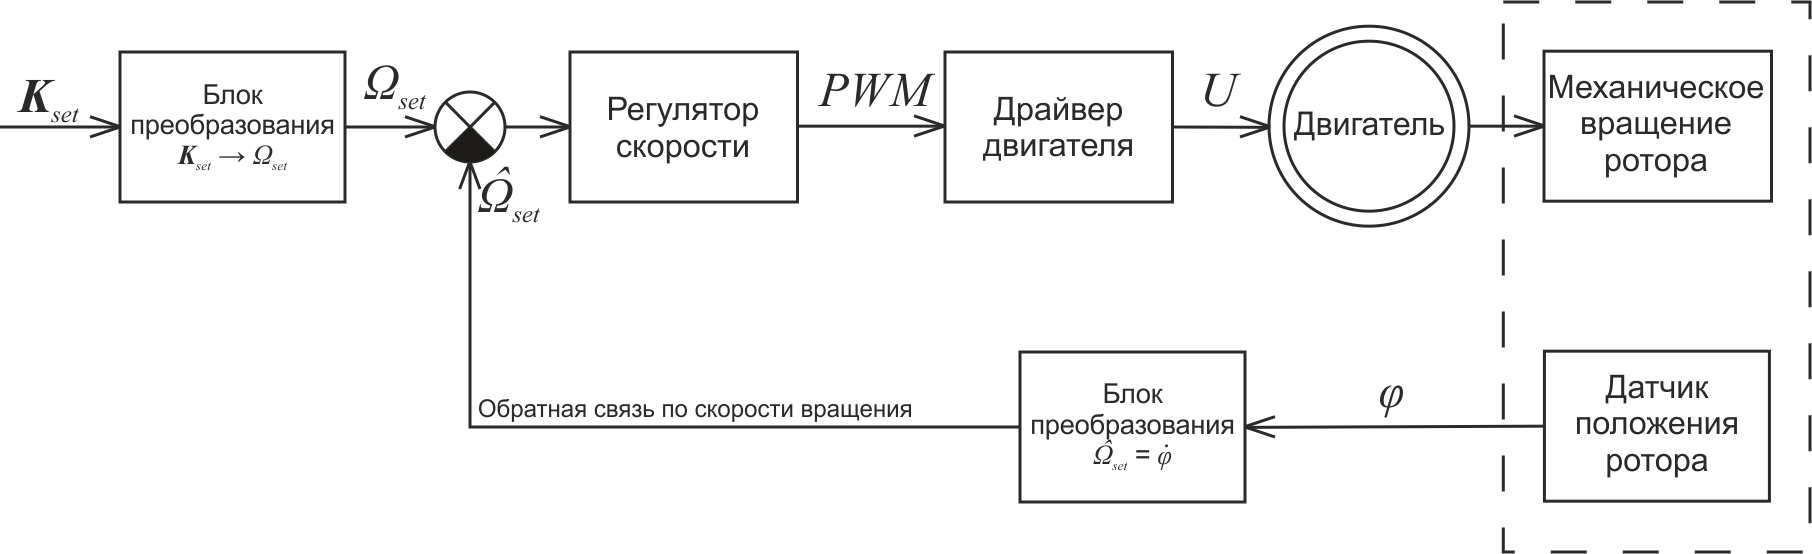
\includegraphics[width=0.9\linewidth]{Control_system.png}%
	\caption{Схема управления отдельным двигателем, где $\bK_{set}$ -- вектор внутреннего гиростатического момента; $\bOm_{set}$ -- угловая скорость вращения двигателя; $\hat{\bOm}_{set}$ -- фактическая скорость вращения двигателя; $PWM$ -- широтно-импульсная модуляция, рассчитаная для заданной скорости вращения; $U$ -- напряжение, подаваемое на двигатель; $\varphi$ -- фактическое положение ротора}
	\label{Control_system}
\end{figure}
